% Options for packages loaded elsewhere
\PassOptionsToPackage{unicode}{hyperref}
\PassOptionsToPackage{hyphens}{url}
%
\documentclass[
]{article}
\usepackage{amsmath,amssymb}
\usepackage{iftex}
\ifPDFTeX
  \usepackage[T1]{fontenc}
  \usepackage[utf8]{inputenc}
  \usepackage{textcomp} % provide euro and other symbols
\else % if luatex or xetex
  \usepackage{unicode-math} % this also loads fontspec
  \defaultfontfeatures{Scale=MatchLowercase}
  \defaultfontfeatures[\rmfamily]{Ligatures=TeX,Scale=1}
\fi
\usepackage{lmodern}
\ifPDFTeX\else
  % xetex/luatex font selection
\fi
% Use upquote if available, for straight quotes in verbatim environments
\IfFileExists{upquote.sty}{\usepackage{upquote}}{}
\IfFileExists{microtype.sty}{% use microtype if available
  \usepackage[]{microtype}
  \UseMicrotypeSet[protrusion]{basicmath} % disable protrusion for tt fonts
}{}
\makeatletter
\@ifundefined{KOMAClassName}{% if non-KOMA class
  \IfFileExists{parskip.sty}{%
    \usepackage{parskip}
  }{% else
    \setlength{\parindent}{0pt}
    \setlength{\parskip}{6pt plus 2pt minus 1pt}}
}{% if KOMA class
  \KOMAoptions{parskip=half}}
\makeatother
\usepackage{xcolor}
\usepackage[margin=1in]{geometry}
\usepackage{color}
\usepackage{fancyvrb}
\newcommand{\VerbBar}{|}
\newcommand{\VERB}{\Verb[commandchars=\\\{\}]}
\DefineVerbatimEnvironment{Highlighting}{Verbatim}{commandchars=\\\{\}}
% Add ',fontsize=\small' for more characters per line
\usepackage{framed}
\definecolor{shadecolor}{RGB}{248,248,248}
\newenvironment{Shaded}{\begin{snugshade}}{\end{snugshade}}
\newcommand{\AlertTok}[1]{\textcolor[rgb]{0.94,0.16,0.16}{#1}}
\newcommand{\AnnotationTok}[1]{\textcolor[rgb]{0.56,0.35,0.01}{\textbf{\textit{#1}}}}
\newcommand{\AttributeTok}[1]{\textcolor[rgb]{0.13,0.29,0.53}{#1}}
\newcommand{\BaseNTok}[1]{\textcolor[rgb]{0.00,0.00,0.81}{#1}}
\newcommand{\BuiltInTok}[1]{#1}
\newcommand{\CharTok}[1]{\textcolor[rgb]{0.31,0.60,0.02}{#1}}
\newcommand{\CommentTok}[1]{\textcolor[rgb]{0.56,0.35,0.01}{\textit{#1}}}
\newcommand{\CommentVarTok}[1]{\textcolor[rgb]{0.56,0.35,0.01}{\textbf{\textit{#1}}}}
\newcommand{\ConstantTok}[1]{\textcolor[rgb]{0.56,0.35,0.01}{#1}}
\newcommand{\ControlFlowTok}[1]{\textcolor[rgb]{0.13,0.29,0.53}{\textbf{#1}}}
\newcommand{\DataTypeTok}[1]{\textcolor[rgb]{0.13,0.29,0.53}{#1}}
\newcommand{\DecValTok}[1]{\textcolor[rgb]{0.00,0.00,0.81}{#1}}
\newcommand{\DocumentationTok}[1]{\textcolor[rgb]{0.56,0.35,0.01}{\textbf{\textit{#1}}}}
\newcommand{\ErrorTok}[1]{\textcolor[rgb]{0.64,0.00,0.00}{\textbf{#1}}}
\newcommand{\ExtensionTok}[1]{#1}
\newcommand{\FloatTok}[1]{\textcolor[rgb]{0.00,0.00,0.81}{#1}}
\newcommand{\FunctionTok}[1]{\textcolor[rgb]{0.13,0.29,0.53}{\textbf{#1}}}
\newcommand{\ImportTok}[1]{#1}
\newcommand{\InformationTok}[1]{\textcolor[rgb]{0.56,0.35,0.01}{\textbf{\textit{#1}}}}
\newcommand{\KeywordTok}[1]{\textcolor[rgb]{0.13,0.29,0.53}{\textbf{#1}}}
\newcommand{\NormalTok}[1]{#1}
\newcommand{\OperatorTok}[1]{\textcolor[rgb]{0.81,0.36,0.00}{\textbf{#1}}}
\newcommand{\OtherTok}[1]{\textcolor[rgb]{0.56,0.35,0.01}{#1}}
\newcommand{\PreprocessorTok}[1]{\textcolor[rgb]{0.56,0.35,0.01}{\textit{#1}}}
\newcommand{\RegionMarkerTok}[1]{#1}
\newcommand{\SpecialCharTok}[1]{\textcolor[rgb]{0.81,0.36,0.00}{\textbf{#1}}}
\newcommand{\SpecialStringTok}[1]{\textcolor[rgb]{0.31,0.60,0.02}{#1}}
\newcommand{\StringTok}[1]{\textcolor[rgb]{0.31,0.60,0.02}{#1}}
\newcommand{\VariableTok}[1]{\textcolor[rgb]{0.00,0.00,0.00}{#1}}
\newcommand{\VerbatimStringTok}[1]{\textcolor[rgb]{0.31,0.60,0.02}{#1}}
\newcommand{\WarningTok}[1]{\textcolor[rgb]{0.56,0.35,0.01}{\textbf{\textit{#1}}}}
\usepackage{graphicx}
\makeatletter
\def\maxwidth{\ifdim\Gin@nat@width>\linewidth\linewidth\else\Gin@nat@width\fi}
\def\maxheight{\ifdim\Gin@nat@height>\textheight\textheight\else\Gin@nat@height\fi}
\makeatother
% Scale images if necessary, so that they will not overflow the page
% margins by default, and it is still possible to overwrite the defaults
% using explicit options in \includegraphics[width, height, ...]{}
\setkeys{Gin}{width=\maxwidth,height=\maxheight,keepaspectratio}
% Set default figure placement to htbp
\makeatletter
\def\fps@figure{htbp}
\makeatother
\setlength{\emergencystretch}{3em} % prevent overfull lines
\providecommand{\tightlist}{%
  \setlength{\itemsep}{0pt}\setlength{\parskip}{0pt}}
\setcounter{secnumdepth}{-\maxdimen} % remove section numbering
\ifLuaTeX
  \usepackage{selnolig}  % disable illegal ligatures
\fi
\IfFileExists{bookmark.sty}{\usepackage{bookmark}}{\usepackage{hyperref}}
\IfFileExists{xurl.sty}{\usepackage{xurl}}{} % add URL line breaks if available
\urlstyle{same}
\hypersetup{
  pdftitle={Overview: Keyword racism},
  pdfauthor={Nathan Alexander},
  hidelinks,
  pdfcreator={LaTeX via pandoc}}

\title{Overview: Keyword \texttt{racism}}
\author{Nathan Alexander}
\date{2024-02-25}

\begin{document}
\maketitle

\hypertarget{google-trend-analysis-of-racism}{%
\section{Google trend analysis of
racism}\label{google-trend-analysis-of-racism}}

We generate a basic analysis of Google Trends data on the term
\texttt{racism}.

\hypertarget{year-google-trend}{%
\subsection{10-year Google Trend}\label{year-google-trend}}

Searches for the term \texttt{racism} in the United States

\begin{Shaded}
\begin{Highlighting}[]
\CommentTok{\# racism (10{-}year trend)}
\NormalTok{racism10year}\OtherTok{\textless{}{-}}\FunctionTok{gtrends}\NormalTok{(}\FunctionTok{c}\NormalTok{(}\StringTok{"racism"}\NormalTok{), }\AttributeTok{time=} \StringTok{"2013{-}01{-}01 2023{-}12{-}31"}\NormalTok{, }\AttributeTok{geo =} \StringTok{"US"}\NormalTok{)}
\FunctionTok{plot}\NormalTok{(racism10year)}
\end{Highlighting}
\end{Shaded}

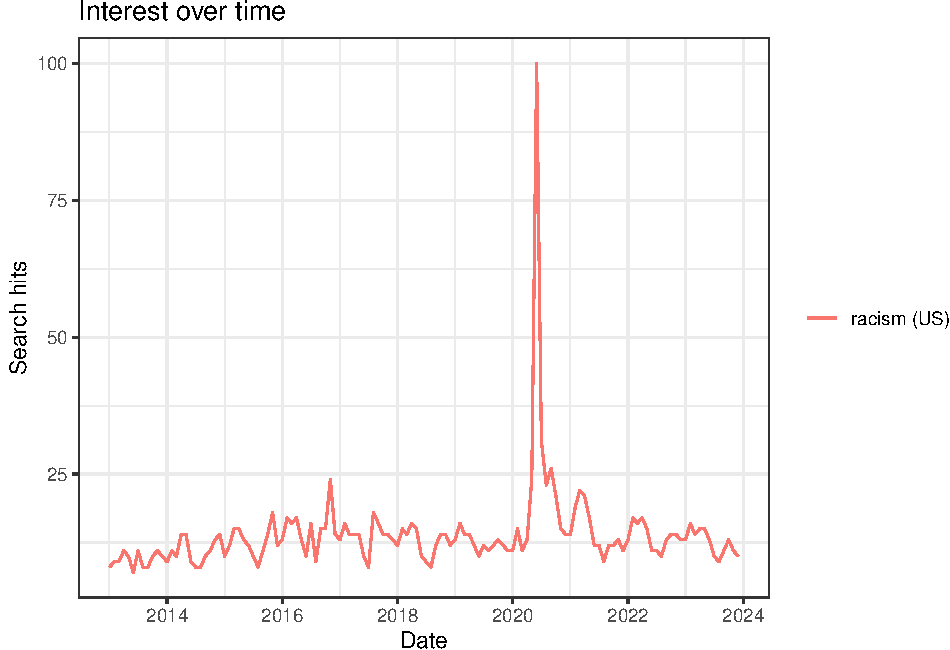
\includegraphics{overview-keyword-racism_files/figure-latex/unnamed-chunk-2-1.pdf}

Hypothesis was a spike in US between 2019 and 2022.

\hypertarget{year-google-trend-for-2020-and-2021}{%
\subsection{2-year Google Trend for 2020 and
2021}\label{year-google-trend-for-2020-and-2021}}

Searches for the term \texttt{racism} in the United States

\begin{Shaded}
\begin{Highlighting}[]
\CommentTok{\# racism (1{-}year trend for 2021)}
\NormalTok{racism1year}\OtherTok{\textless{}{-}}\FunctionTok{gtrends}\NormalTok{(}\FunctionTok{c}\NormalTok{(}\StringTok{"racism"}\NormalTok{), }\AttributeTok{time=} \StringTok{"2019{-}12{-}31 2021{-}12{-}31"}\NormalTok{, }\AttributeTok{geo =} \StringTok{"US"}\NormalTok{)}
\FunctionTok{plot}\NormalTok{(racism1year)}
\end{Highlighting}
\end{Shaded}

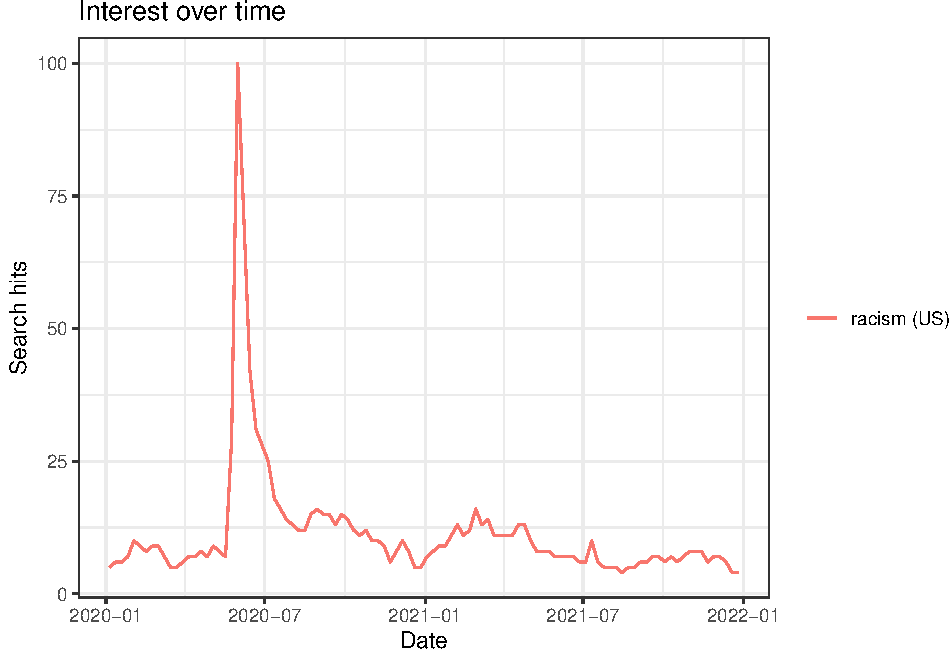
\includegraphics{overview-keyword-racism_files/figure-latex/unnamed-chunk-3-1.pdf}

\hypertarget{search-for-racism-and-covid}{%
\subsection{\texorpdfstring{Search for \texttt{racism} and
\texttt{covid}}{Search for racism and covid}}\label{search-for-racism-and-covid}}

Adding 10-year historical context (Covid) to searches for racism

\begin{Shaded}
\begin{Highlighting}[]
\NormalTok{racism\_covid}\OtherTok{\textless{}{-}}\FunctionTok{gtrends}\NormalTok{(}\FunctionTok{c}\NormalTok{(}\StringTok{"covid"}\NormalTok{, }\StringTok{"racism"}\NormalTok{), }\AttributeTok{time=} \StringTok{"2013{-}01{-}01 2023{-}12{-}31"}\NormalTok{, }\AttributeTok{geo =} \StringTok{"US"}\NormalTok{)}
\FunctionTok{plot}\NormalTok{(racism\_covid)}
\end{Highlighting}
\end{Shaded}

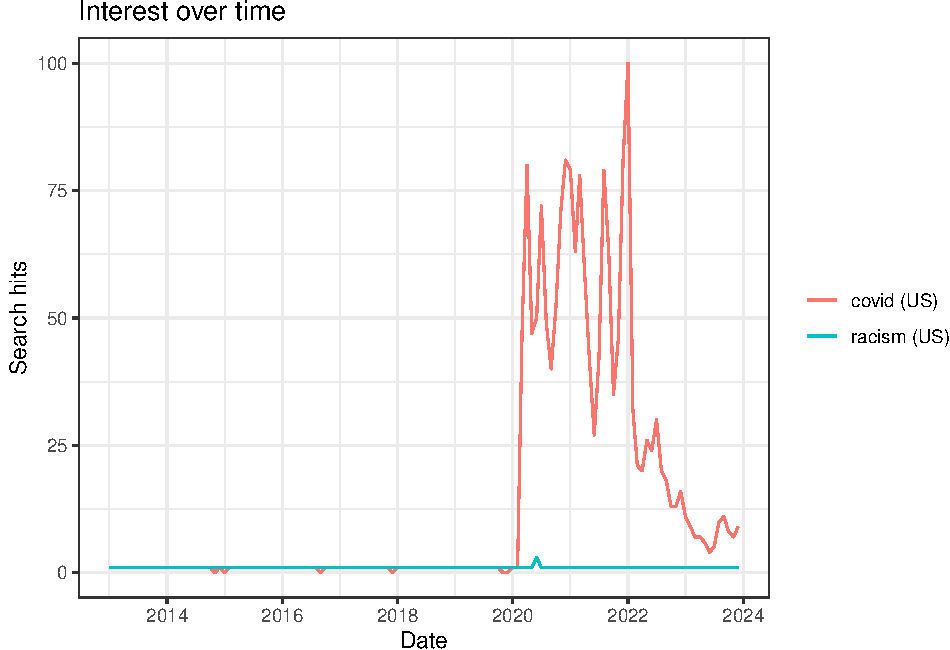
\includegraphics{overview-keyword-racism_files/figure-latex/unnamed-chunk-4-1.pdf}

\hypertarget{search-for-racism-and-stem}{%
\subsection{\texorpdfstring{Search for \texttt{racism} and
\texttt{stem}}{Search for racism and stem}}\label{search-for-racism-and-stem}}

Adding 10-year ancillary context (subject=stem) to searches for racism

\begin{Shaded}
\begin{Highlighting}[]
\NormalTok{racism\_stem}\OtherTok{\textless{}{-}}\FunctionTok{gtrends}\NormalTok{(}\FunctionTok{c}\NormalTok{(}\StringTok{"stem"}\NormalTok{, }\StringTok{"racism"}\NormalTok{), }\AttributeTok{time=} \StringTok{"2013{-}01{-}01 2023{-}12{-}31"}\NormalTok{, }\AttributeTok{geo =} \StringTok{"US"}\NormalTok{)}
\FunctionTok{plot}\NormalTok{(racism\_stem)}
\end{Highlighting}
\end{Shaded}

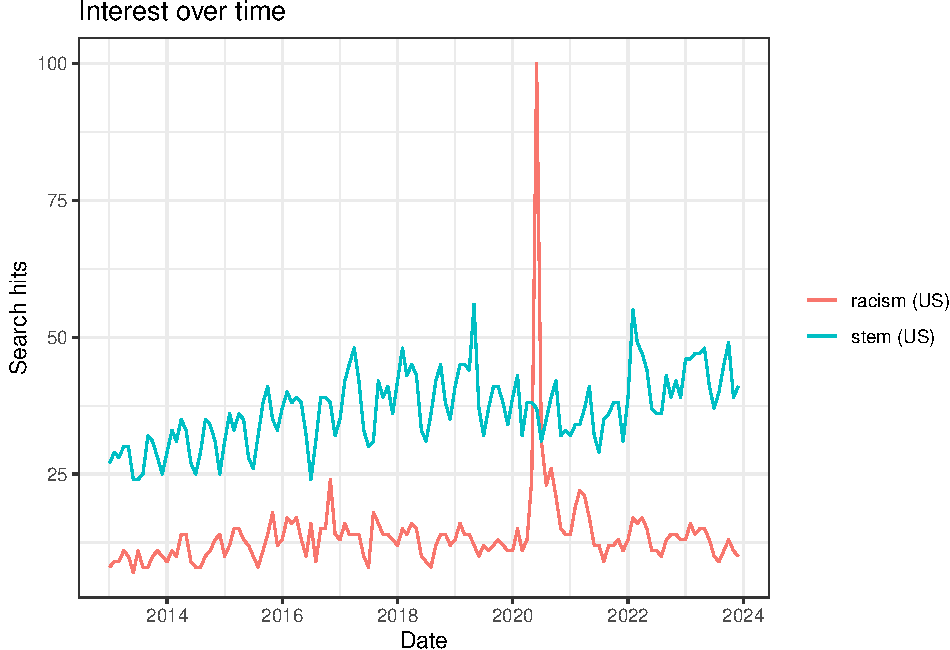
\includegraphics{overview-keyword-racism_files/figure-latex/unnamed-chunk-5-1.pdf}

\hypertarget{search-for-racism-and-education}{%
\subsection{\texorpdfstring{Search for \texttt{racism} and
\texttt{education}}{Search for racism and education}}\label{search-for-racism-and-education}}

Adding 10-year ancillary context (subject=education) to searches for
racism

\begin{Shaded}
\begin{Highlighting}[]
\NormalTok{racism\_education}\OtherTok{\textless{}{-}}\FunctionTok{gtrends}\NormalTok{(}\FunctionTok{c}\NormalTok{(}\StringTok{"education"}\NormalTok{, }\StringTok{"racism"}\NormalTok{), }\AttributeTok{time=} \StringTok{"2013{-}01{-}01 2023{-}12{-}31"}\NormalTok{, }\AttributeTok{geo =} \StringTok{"US"}\NormalTok{)}
\FunctionTok{plot}\NormalTok{(racism\_education)}
\end{Highlighting}
\end{Shaded}

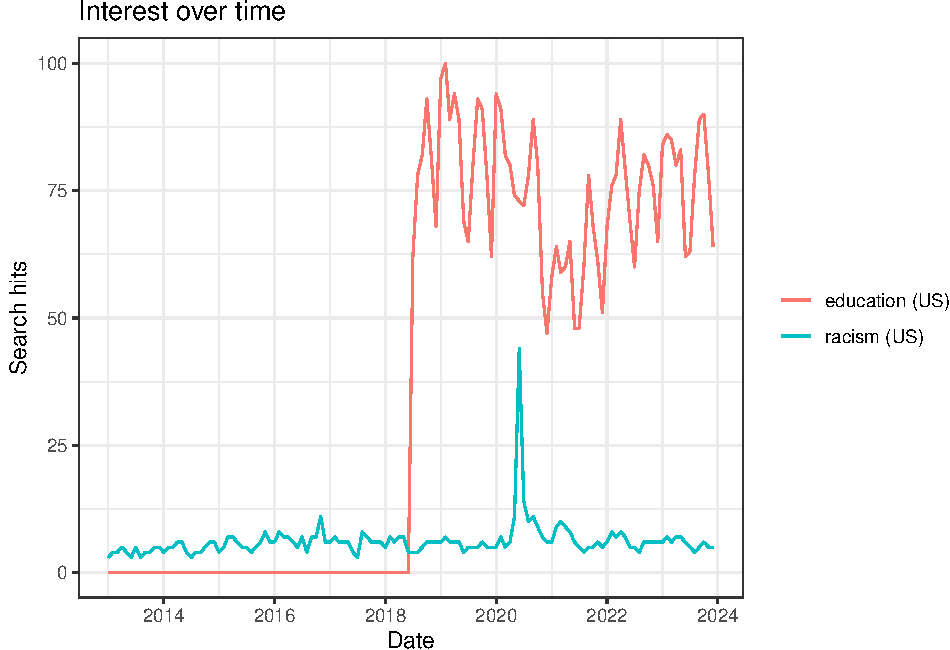
\includegraphics{overview-keyword-racism_files/figure-latex/unnamed-chunk-6-1.pdf}

\hypertarget{search-for-racism-and-george-floyd}{%
\subsection{\texorpdfstring{Search for \texttt{racism} and
\texttt{george\ floyd}}{Search for racism and george floyd}}\label{search-for-racism-and-george-floyd}}

Adding historical context (person=george floyd) to searches for racism

\begin{Shaded}
\begin{Highlighting}[]
\NormalTok{racism\_george\_floyd}\OtherTok{\textless{}{-}}\FunctionTok{gtrends}\NormalTok{(}\FunctionTok{c}\NormalTok{(}\StringTok{"george floyd"}\NormalTok{, }\StringTok{"racism"}\NormalTok{), }\AttributeTok{time=} \StringTok{"2019{-}12{-}31 2021{-}12{-}31"}\NormalTok{, }\AttributeTok{geo =} \StringTok{"US"}\NormalTok{)}
\FunctionTok{plot}\NormalTok{(racism\_george\_floyd)}
\end{Highlighting}
\end{Shaded}

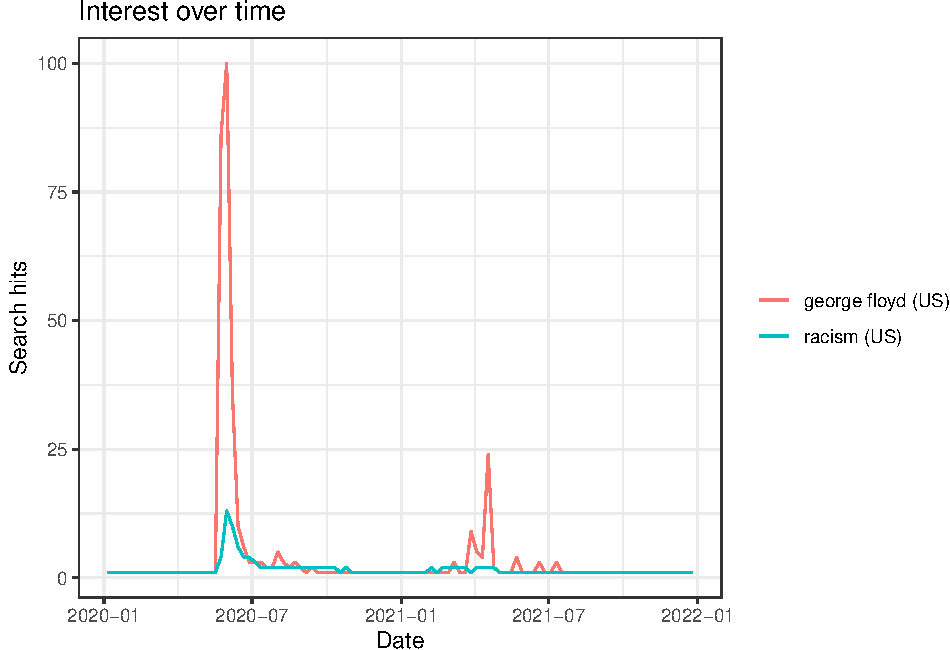
\includegraphics{overview-keyword-racism_files/figure-latex/unnamed-chunk-7-1.pdf}

\begin{Shaded}
\begin{Highlighting}[]
\NormalTok{racism\_george\_floyd}\OtherTok{\textless{}{-}}\FunctionTok{gtrends}\NormalTok{(}\FunctionTok{c}\NormalTok{(}\StringTok{"george floyd"}\NormalTok{, }\StringTok{"racism"}\NormalTok{), }\AttributeTok{time=} \StringTok{"2019{-}12{-}31 2021{-}12{-}31"}\NormalTok{, }\AttributeTok{geo =} \StringTok{"US"}\NormalTok{)}

\NormalTok{racism\_george\_floyd\_2 }\OtherTok{\textless{}{-}}\NormalTok{ racism\_george\_floyd}\SpecialCharTok{$}\NormalTok{interest\_over\_time }\SpecialCharTok{\%\textgreater{}\%} 
\NormalTok{  dplyr}\SpecialCharTok{::}\FunctionTok{mutate}\NormalTok{(}\AttributeTok{hits=}\FunctionTok{ifelse}\NormalTok{(hits}\SpecialCharTok{==}\StringTok{"\textless{}1"}\NormalTok{,}\FloatTok{0.5}\NormalTok{, }\FunctionTok{as.numeric}\NormalTok{(hits)),}
         \AttributeTok{date=}\FunctionTok{as.Date}\NormalTok{(date))}
\end{Highlighting}
\end{Shaded}

\begin{verbatim}
## Warning: There was 1 warning in `dplyr::mutate()`.
## i In argument: `hits = ifelse(hits == "<1", 0.5, as.numeric(hits))`.
## Caused by warning in `ifelse()`:
## ! NAs introduced by coercion
\end{verbatim}

\begin{Shaded}
\begin{Highlighting}[]
\FunctionTok{ggplot}\NormalTok{(racism\_george\_floyd\_2, }\FunctionTok{aes}\NormalTok{(}\AttributeTok{x=}\NormalTok{date, }\AttributeTok{y=}\NormalTok{hits, }\AttributeTok{color=}\NormalTok{keyword)) }\SpecialCharTok{+}
  \FunctionTok{geom\_line}\NormalTok{() }\SpecialCharTok{+}
  \FunctionTok{geom\_vline}\NormalTok{(}\AttributeTok{xintercept=}\FunctionTok{as.numeric}\NormalTok{(}\FunctionTok{as.Date}\NormalTok{(}\StringTok{"2020{-}05{-}25"}\NormalTok{)))}
\end{Highlighting}
\end{Shaded}

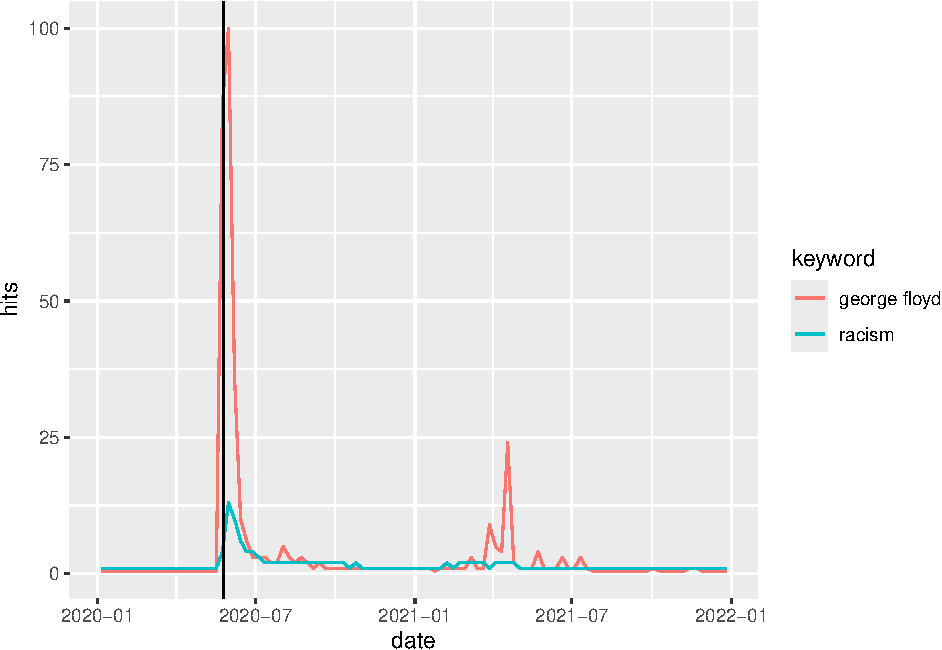
\includegraphics{overview-keyword-racism_files/figure-latex/unnamed-chunk-8-1.pdf}

\hypertarget{add-date-of-george-floyd-murder-by-police}{%
\subsection{Add date of George Floyd murder by
police}\label{add-date-of-george-floyd-murder-by-police}}

Layering date of George Floyd's murder (may 25, 2020) to plot.

\begin{Shaded}
\begin{Highlighting}[]
\NormalTok{racism1year}\OtherTok{\textless{}{-}}\FunctionTok{gtrends}\NormalTok{(}\FunctionTok{c}\NormalTok{(}\StringTok{"racism"}\NormalTok{, }\StringTok{"george floyd"}\NormalTok{, }\StringTok{"covid"}\NormalTok{), }\AttributeTok{time=} \StringTok{"2019{-}12{-}31 2021{-}12{-}31"}\NormalTok{, }\AttributeTok{geo =} \StringTok{"US"}\NormalTok{)}

\NormalTok{racism1year\_trend }\OtherTok{\textless{}{-}}\NormalTok{ racism1year}\SpecialCharTok{$}\NormalTok{interest\_over\_time }\SpecialCharTok{\%\textgreater{}\%} 
\NormalTok{  dplyr}\SpecialCharTok{::}\FunctionTok{mutate}\NormalTok{(}\AttributeTok{hits=}\FunctionTok{ifelse}\NormalTok{(hits}\SpecialCharTok{==}\StringTok{"\textless{}1"}\NormalTok{,}\FloatTok{0.5}\NormalTok{, }\FunctionTok{as.numeric}\NormalTok{(hits)),}
         \AttributeTok{date=}\FunctionTok{as.Date}\NormalTok{(date))}
\end{Highlighting}
\end{Shaded}

\begin{verbatim}
## Warning: There was 1 warning in `dplyr::mutate()`.
## i In argument: `hits = ifelse(hits == "<1", 0.5, as.numeric(hits))`.
## Caused by warning in `ifelse()`:
## ! NAs introduced by coercion
\end{verbatim}

\begin{Shaded}
\begin{Highlighting}[]
\FunctionTok{ggplot}\NormalTok{(racism1year\_trend, }\FunctionTok{aes}\NormalTok{(}\AttributeTok{x=}\NormalTok{date, }\AttributeTok{y=}\NormalTok{hits, }\AttributeTok{color=}\NormalTok{keyword)) }\SpecialCharTok{+}
  \FunctionTok{geom\_line}\NormalTok{() }\SpecialCharTok{+}
  \FunctionTok{geom\_vline}\NormalTok{(}\AttributeTok{xintercept=}\FunctionTok{as.numeric}\NormalTok{(}\FunctionTok{as.Date}\NormalTok{(}\StringTok{"2020{-}05{-}25"}\NormalTok{)))}
\end{Highlighting}
\end{Shaded}

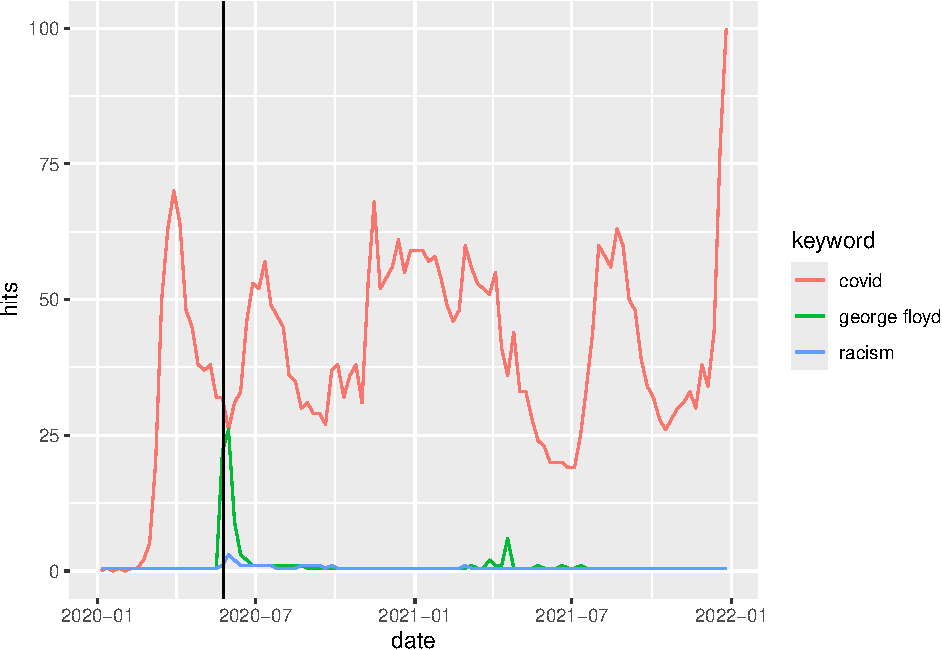
\includegraphics{overview-keyword-racism_files/figure-latex/unnamed-chunk-9-1.pdf}

The above information will inform our keyword inquiries for a
bibliometric analysis.

\end{document}
